%%
% このファイルは、筑波大学情報学群情報科学類の
% 卒業研究論文本体のサンプルです。
% このファイルを書き換えて、この例と同じような書式の論文本体を
% LaTeXを使って作成することができます。
% 
% PC環境や、LaTeX環境の設定によっては漢字コードや改行コードを
% 変更する必要があります。
%%
\documentclass[a4paper,11pt,dvipdfmx]{jreport}

%%【PostScript, JPEG, PNG等の画像の貼り込み】
%% 利用するパッケージを選んでコメントアウトしてください。
\usepackage{graphicx} % for \includegraphics[width=3cm]{sample.eps}
%\usepackage{epsfig} % for \psfig{file=sample.eps,width=3cm}
%\usepackage{epsf} % for \epsfile{file=sample.eps,scale=0.6}
%\usepackage{epsbox} % for \epsfile{file=sample.eps,scale=0.6}

%% dvipdfm を使う場合(dvi->pdfを直接生成する場合)
%\usepackage[dvipdfm]{color,graphicx}
%% dvipdfm を使ってPDFの「しおり」を付ける場合
%\usepackage[dvipdfm,bookmarks=true,bookmarksnumbered=true,bookmarkstype=toc]{hyperref}
%% 参考:dvipdfm 日本語版
%% http://hamilcar.phys.kyushu-u.ac.jp/~hirata/dvipdfm/

\usepackage[bookmarksnumbered=true]{hyperref}
\usepackage{pxjahyper}

\usepackage{times} % use Times Font instead of Computer Modern

\setcounter{tocdepth}{3}
\setcounter{page}{-1}

\setlength{\oddsidemargin}{0.1in}
\setlength{\evensidemargin}{0.1in} 
\setlength{\topmargin}{0in}
\setlength{\textwidth}{6in} 
%\setlength{\textheight}{10.1in}
\setlength{\parskip}{0em}
\setlength{\topsep}{0em}

%\newcommand{\zu}[1]{{\gt \bf 図\ref{#1}}}

%% タイトル生成用パッケージ(重要)
\usepackage{coins-jp}
\usepackage{jumoline}

%% タイトル
%% 【注意】タイトルの最後に\\ を入れるとエラーになります
\title{\Underline{レキシカル環境にメソッドを定義する\\オブジェクト指向言語Suzu}}
%% 著者
\author{林 拓人}
%% 指導教員
\advisor{前田敦司}

%% 専攻名 と 年月 (提出年月)
%% 年月は必要に応じて書き替えてください。
\heiseiyear{26}  % 平成の年度
\majorfield{ソフトウェアサイエンス主専攻}
%\majorfield{情報システム主専攻}
%\majorfield{知能情報メディア主専攻}

\makeatletter%% プリアンブルで定義する場合は必須

%% (j)report・(j)book クラスの場合
%% 
\renewenvironment{thebibliography}[1]% 再定義
{\chapter*{\bibname\@mkboth{\bibname}{\bibname}}%
	\addcontentsline{toc}{chapter}{\numberline{}\bibname}% この行追加
	\list{\@biblabel{\@arabic\c@enumiv}}%
	{\settowidth\labelwidth{\@biblabel{#1}}%
		\leftmargin\labelwidth
		\advance\leftmargin\labelsep
		\@openbib@code
		\usecounter{enumiv}%
		\let\p@enumiv\@empty
		\renewcommand\theenumiv{\@arabic\c@enumiv}}%
	\sloppy
	\clubpenalty4000
	\@clubpenalty\clubpenalty
	\widowpenalty4000%
	\sfcode`\.\@m}
{\def\@noitemerr
	{\@latex@warning{Empty `thebibliography' environment}}%
	\endlist}

\makeatother%% プリアンブルで定義する場合は必須


\begin{document}
\maketitle
\thispagestyle{empty}
\newpage

\thispagestyle{empty}
\vspace*{20pt plus 1fil}
\parindent=1zw
\noindent
%%
%% 論文の概要(Abstract)
%%
\begin{center}
{\Large \bf 要  旨}
\vspace{2cm}
\end{center}
%400字程度
従来のクラスベース・オブジェクトシステムは,メソッドをクラスに格納するものと総称関数に格納するもの
(メソッドがクラスに属すものと総称関数に属すもの)とに分けられる.
本論文はこれらのいずれとも異なり,環境にメソッドを直接格納する新しいオブジェクトシステムを
提案する.
クラスや総称関数といった枠を廃し,クラス名とメソッド名の組をキーとして環境にメソッドを直接格納する.
これにより変数に対して行えるあらゆる操作がメソッドに対しても自然に行えるようになり,従来の方式に比べ
シンプルな仕組みで柔軟なオブジェクト指向プログラミングが可能となる.
提案する手法の有用性を実証するため,このオブジェクトシステムを搭載する独自言語Suzuの処理系を
実装した.
Suzuの特徴を生かすプログラム例として言語内DSL(Domain Specific Language)の構築例を挙げる.
従来のオブジェクトシステムにおける類似した概念等との関連についても議論する.


%%%%%
\par
\vspace{0pt plus 1fil}
\newpage

\pagenumbering{roman} % I, II, III, IV 
\tableofcontents
\listoffigures
%\listoftables

\pagebreak \setcounter{page}{1}
\pagenumbering{arabic} % 1,2,3


\chapter{序論}

従来のクラスベース・オブジェクトシステムは,メソッドの格納方式をモデル化すると
次の2つのモデルに分類することができる.
1つはクラスにメソッドを格納するモデル,もう1つはCLOS\cite{Ida:2010}のように
総称関数にメソッドを格納するモデルである.

本論文は,これら2つの格納モデルに対する分析に基づき考案した,全く新しい格納モデルを持つ
オブジェクトシステムを提案する.
また,その特徴を最大限に生かせるよう独自に設計したプログラミング言語Suzuを用いて,提案する
オブジェクトシステムの評価を行う.

なお,ここでのモデルとはプログラミング言語が仕様上オブジェクトシステムをどうとらえているかを
表すものであり,特定の実装方法を指すものではない.
オブジェクトシステムに対し従来とは異なる新たな見方を提供することで,有用と思われる機能に
自然な意味付けを与えたり,既存の概念を整理したりといった目的を持つものである.


\chapter{オブジェクトシステムのモデル化}

\section{従来のオブジェクトシステム}

ここではモデルを単純化するため,単一ディスパッチ(1つのオブジェクトに基づきメソッドを決定する方式)
の場合についてのみ考える.
多重ディスパッチ(複数のオブジェクトに基づきメソッドを決定する方式)へのモデルの拡張については
\ref{section:multiple-dispatch}節で検討する.

\subsection{クラスにメソッドを格納するモデル}
\label{section:classes}

クラスにメソッドを格納するモデルでは環境(名前と値の束縛の集合)にクラスを格納し,
クラスにメソッドを格納する(図\ref{figure:classes}).
ここで環境はクラス名をキーとしてクラスを格納する辞書であり,クラスはメソッド名をキーとして
メソッドを格納する辞書である.
SmalltalkやRubyといった言語のオブジェクトシステムはこのモデルに分類される.

\begin{figure}[htbp]
	\centering
	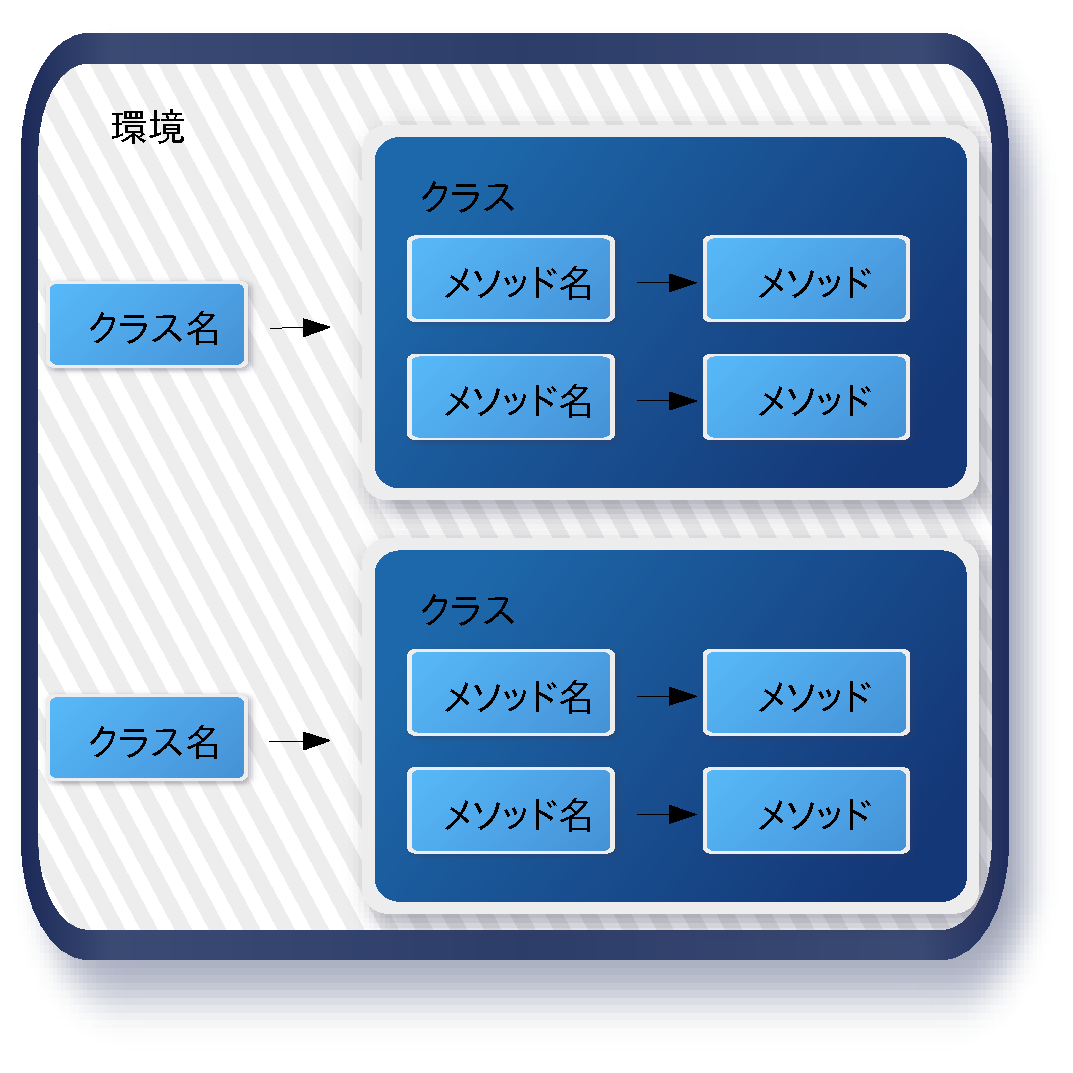
\includegraphics[width=6.5cm]{fig/classes-crop.pdf}
	\caption{クラスにメソッドを格納するモデル}
	\label{figure:classes}
\end{figure}

\subsection{総称関数にメソッドを格納するモデル}
\label{section:generic-finctions}

総称関数にメソッドを格納するモデルでは環境に総称関数を格納し,総称関数にメソッドを格納する
(図\ref{figure:generic-functions}).
ここで環境はメソッド名をキーとして総称関数を格納する辞書であり,総称関数はクラス名をキーとして
メソッドを格納する辞書である.
単一ディスパッチに限定したCLOSはこのモデルに分類される.

\begin{figure}[htbp]
	\centering
	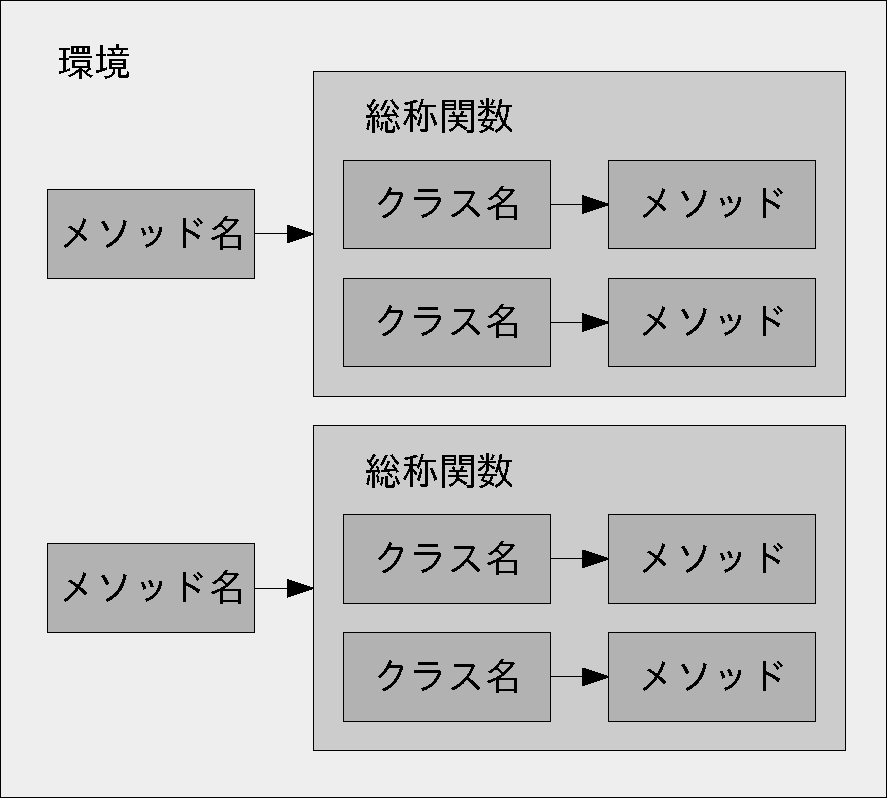
\includegraphics[width=6.5cm]{fig/generic-functions-crop.pdf}
	\caption{総称関数にメソッドを格納するモデル}
	\label{figure:generic-functions}
\end{figure}

\section{提案するオブジェクトシステム}
\label{section:proposal}

従来のオブジェクトシステムの分類先である2つのモデルでは,どちらもクラス名とメソッド名が決まれば
メソッドが一意に定まることが要請されている.
また,環境という辞書の中にクラスあるいは総称関数という辞書が入れ子になっている構造も
共通している.

提案するオブジェクトシステムはこのようなクラスや総称関数による入れ子構造を廃し,
\textbf{環境にメソッドを直接格納するモデル}を採用する(図\ref{figure:environment}).
ここで環境は\textbf{クラス名とメソッド名の組}をキーとしてメソッドを格納する辞書である.

\begin{figure}[htbp]
	\centering
	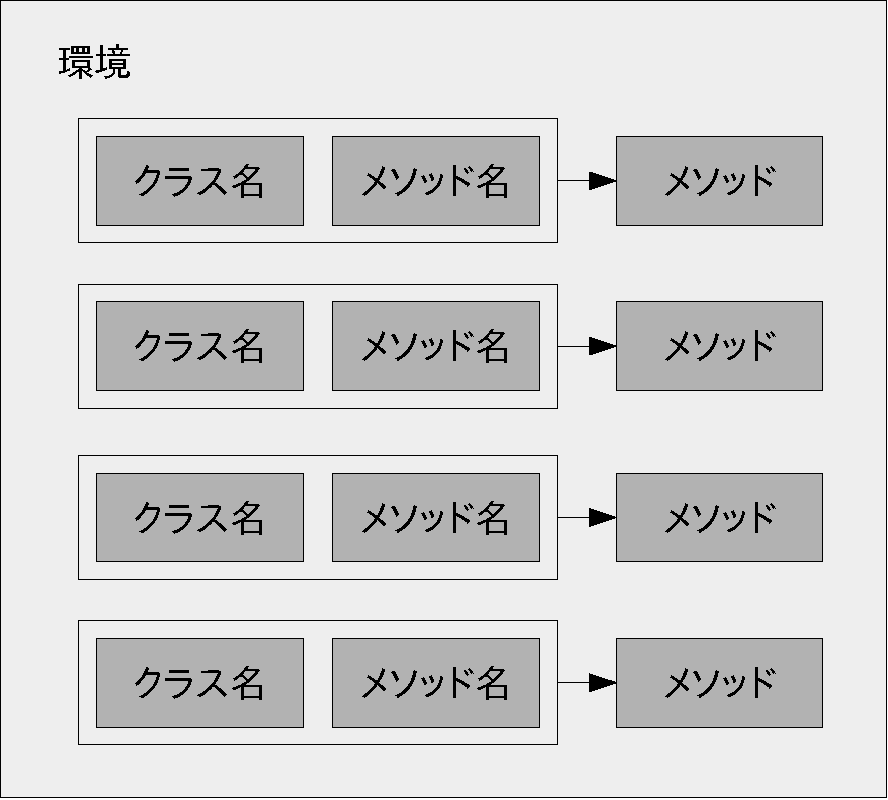
\includegraphics[width=6.5cm]{fig/environment-crop.pdf}
	\caption{環境にメソッドを直接格納するモデル}
	\label{figure:environment}
\end{figure}

このモデルの特徴は,メソッドの格納方式が一般的な変数の格納方式と類似していることである.
メソッドがクラス名とメソッド名の組をキーとして環境に格納されるのに対し,変数は変数名を
キーとして環境に格納される.

これはすなわち,「変数名」を「クラス名とメソッド名の組」に置き換えることで,
\textbf{変数に対して行えるあらゆる操作がメソッドに対しても自然に行える(自然な意味付けが可能である)}
ということである.
具体的には,ローカル変数に対応する\textbf{ローカルメソッド}の定義,シャドーイング,
モジュールからのエクスポート・インポート,仮引数としての指定などが挙げられる.
第\ref{chapter:suzu}章では提案するオブジェクトシステムを搭載した独自の
プログラミング言語Suzuを用いて,この特徴を生かした実際のプログラム例を示す.


\chapter{プログラミング言語Suzu}
\label{chapter:suzu}

環境にメソッドを直接格納するモデルに基づき設計した独自のプログラミング言語Suzuの解説とその
プログラム例により,提案するオブジェクトシステムの有用性を示す.

\section{基本的な文法}

\verb|//|から行末まではコメントである.
以降,\verb|//=>|に続くコメントはプログラムの出力を表すものとする.
出力にはデバッグ用出力関数\verb|p|を用いる.

変数を定義するには\verb|let x = 123|のようにする.
ここでは変数\verb|x|に整数値\verb|123|を代入している.

関数呼び出しは\verb|func(arg1, arg2)|のようにする.
ここでは関数\verb|func|を第1引数\verb|arg1|,第2引数\verb|arg2|で呼び出している.

関数定義は以下のようにする.
\begin{quote}
	\begin{verbatim}
	def fac(n):
	if(n == 0):
	1
	else:
	n * fac(n - 1)
	end
	end
	\end{verbatim}
\end{quote}
これは以下のコードと意味的に等価である.
\begin{quote}
	\begin{verbatim}
	let fac = ^(n):
	if(n == 0):
	1
	else:
	n * fac(n - 1)
	end
	end
	\end{verbatim}
\end{quote}
\verb|^(n):|から\verb|end|までの部分は引数\verb|n|を受け取って\verb|end|までの
式を評価する関数リテラルである.\verb|^(n){ ... }|と書くこともできる.

関数リテラルは関数呼び出しの後ろに続けて書くことで追加の引数として高階関数に渡すことができる.
例えば
\begin{quote}
	\begin{verbatim}
	map(lst)^(n):
	n * 2
	end
	\end{verbatim}
\end{quote}
は
\begin{quote}
	\begin{verbatim}
	map(lst, ^(n){ n * 2 })
	\end{verbatim}
\end{quote}
と等価である.

\verb|begin|は新たなスコープを導入し\verb|end|までの式を評価する.
\begin{quote}
	\begin{verbatim}
	let str = "global"
	begin:
	let str = "local"
	p(str)  //=> "local"
	end
	p(str)  //=> "global"
	\end{verbatim}
\end{quote}
Suzuでは\verb|:|と\verb|end|(または\verb|{|と\verb|}|)で囲まれた箇所を
\textbf{ブロック}と呼ぶ.
ブロックには新たなスコープが導入される.

\section{オブジェクトシステム}

ここでは\ref{section:proposal}節で提示したモデルのSuzuにおける具体的な実装を述べる.

クラス名とメソッド名の組は\verb|C#m|と書く.\verb|C|はクラス名,\verb|m|は
メソッド名である.

クラス定義は以下のようにして行う.
\begin{quote}
	\begin{verbatim}
	class Vector:
	def MkVector(x, y)
	end
	\end{verbatim}
\end{quote}
これにより,クラス\verb|Vector|とそのコンストラクタ\verb|MkVector|が定義される.

メソッドは以下のようにクラスとは独立して定義する.仮引数ではコンストラクタ等を用いた
パターンマッチングが使用できる,
第1引数はメソッド呼び出しの対象となったオブジェクト自身,第2引数以降は与えられた実引数となる.
\begin{quote}
	\begin{verbatim}
	def Vector#add(MkVector(x1, y1),
	MkVector(x2, y2)):
	MkVector(x1 + x2, y1 + y2)
	end
	\end{verbatim}
\end{quote}
これは通常の関数定義における変数名をクラス名とメソッド名の組に置き換えた形となっている.
変数と同様\verb|let|を用いた書き方も可能である.

メソッドは\verb|obj.m(arg1, arg2)|のようにして呼び出す.
先程述べたように,メソッドとして呼び出される関数には第1引数として\verb|obj|,
第2・第3引数として\verb|arg1|,\verb|arg2|が渡される.
以下の\verb|a.add(b)|という呼び出しでは上の例で定義した\verb|Vector#add|に,
第1引数として\verb|a|,第2引数として\verb|b|が渡される.
\begin{quote}
	\begin{verbatim}
	let a = MkVector(1, 2)
	let b = MkVector(3, 4)
	p(a.add(b))  //=> MkVector(4, 6)
	\end{verbatim}
\end{quote}
また,独自の演算子をメソッドとして定義することもできる.
二項演算子の場合,左辺がメソッド呼び出しの対象となるオブジェクト,右辺が実引数となる.
\begin{quote}
	\begin{verbatim}
	let Vector#(+) = Vector#add
	p(a + b)  //=> MkVector(4, 6)
	\end{verbatim}
\end{quote}

Suzuは\ref{section:proposal}節で述べた環境にメソッドを直接格納するモデルを採用しているため,
ネストしたスコープの内側にメソッドを定義することで,ローカル変数に対応するローカルメソッドを
ごく自然に定義できる.
\begin{quote}
	\begin{verbatim}
	let v = MkVector(5, 6)
	def Vector#m(self):
	p("global")
	end
	begin:
	def Vector#m(self):
	p("local")
	end
	v.m  //=> "local"
	end
	v.m  //=> "global"
	\end{verbatim}
\end{quote}
このように,メソッドの探索は内側のスコープから順に行われるため,メソッドを変数のように
シャドーイングすることが可能である.

メソッド呼び出しの手順を図に表わすと図\ref{figure:method-call}のようになる.
\verb|a.f(...)|というメソッド呼び出しは次の3ステップを経て実行される.
\begin{enumerate}
	\item \verb|a|からクラス名\verb|A|を取り出してメソッド名\verb|f|と組にする
	\item 組をキーとして環境をルックアップしメソッド\verb|<method>|を発見
	\item 第一引数に\verb|a|を追加し\verb|<method>|を呼び出す
\end{enumerate}

\begin{figure}[htbp]
	\centering
	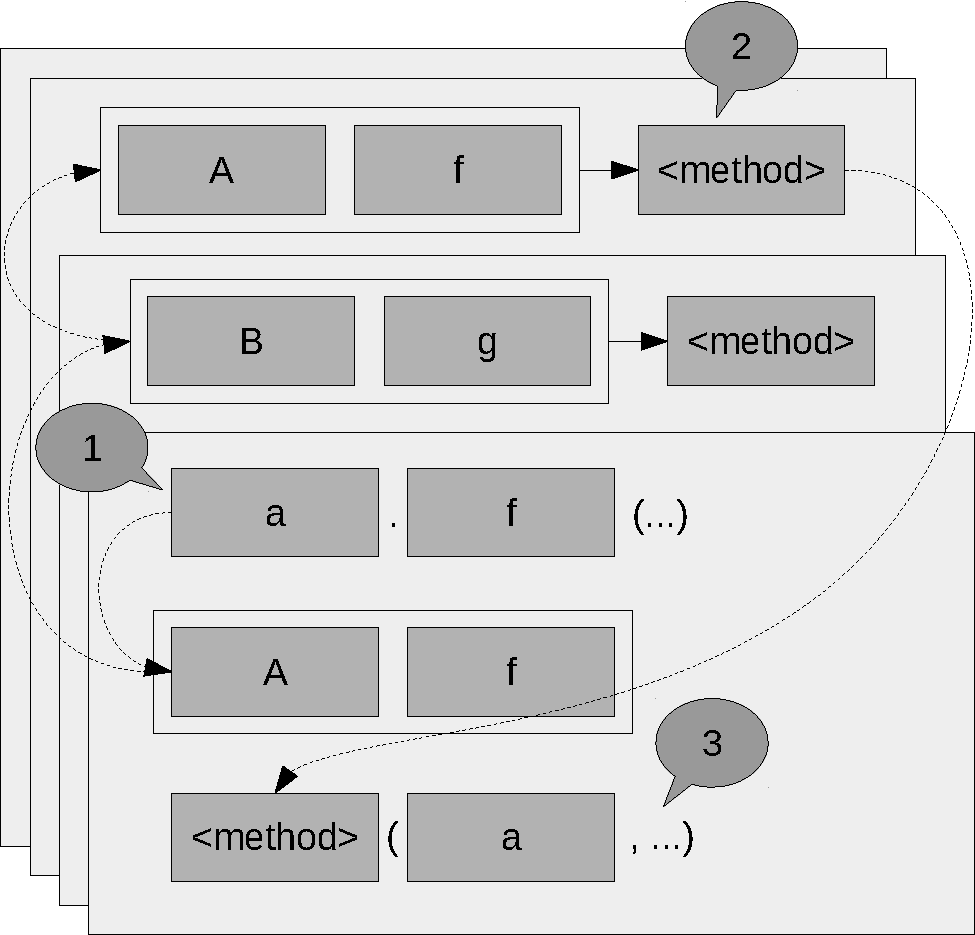
\includegraphics[width=6.5cm]{fig/method-call-crop.pdf}
	\caption{メソッド呼び出しの手順}
	\label{figure:method-call}
\end{figure}

\section{モジュールとトレイト}

Suzuのオブジェクトシステムと調和するモジュールシステムについて述べる.

Suzuのモジュールは他の言語における変数のようにメソッドを個別にエクスポートできる.
\begin{quote}
	\begin{verbatim}
	module A:
	def f(...):
	...
	end
	def C#m(...):
	...
	end
	def C#n(...):
	...
	end
	export f, C#m
	end
	\end{verbatim}
\end{quote}
上の例ではモジュール\verb|A|は変数\verb|f|とメソッド\verb|C#m|をエクスポートするが,
\verb|C#n|はエクスポートしない.
エクスポートされた変数やメソッドは\verb|::|を用いて,\verb|A::f|,\verb|A::(C#m)|
のように参照できる.

モジュールは\verb|open|キーワードを用いて\verb|open|することができる.
モジュールを\verb|open|するとエクスポートされている変数やメソッドがそのスコープで
直接定義されたようにインポートされる.
また,\verb|except|キーワードを用いてインポートの対象から除外することもできる.
\begin{quote}
	\begin{verbatim}
	module B:
	...
	export f, g, C#m, C#n
	end
	begin:
	open B except g, C#n
	...
	end
	\end{verbatim}
\end{quote}
上の例では\verb|begin|から\verb|end|までのスコープで,
モジュール\verb|B|でエクスポートされているもののうち\verb|g|と\verb|C#n|を除いて
インポートを行っている.
これによりスコープ内で\verb|f|と\verb|C#m|を\verb|B::|という修飾子なしに参照できるようになる.

Suzuは継承機構を持たず,実装の再利用はトレイト\cite{Scharli:2003}を用いて行う.
ただし,Suzuのトレイトはそのオブジェクトシステムに適合するよう他の言語と比べて多少
趣の異なるものとなっている.
\begin{quote}
	\begin{verbatim}
	trait T(C, C#m, C#n):
	def C#o(self, ...):
	...
	self.m(...)
	...
	end
	def C#p(self, ...):
	...
	self.n(...)
	...
	end
	export C#o, C#p
	end
	\end{verbatim}
\end{quote}
トレイトは\textbf{クラスやメソッドを受け取ってモジュールを返す関数}として表現される.
上の例では\verb|C#m|や\verb|C#n|のように仮引数としてメソッドを指定している.
使用する側は以下のようにする.
\begin{quote}
	\begin{verbatim}
	open T(D, D#m, D#n)
	open T(E, E#m, E#n)
	\end{verbatim}
\end{quote}
トレイトは既存のクラスとメソッドを受け取って新たなメソッドが定義されたモジュールを生成する.
これを\verb|open|することでメソッドがそのスコープで有効になる.
この例では,\verb|D#o|,\verb|D#p|,\verb|E#o|,\verb|E#p|が新たに定義される.

トレイト同士の加算は単に\verb|open|を並べればよい.メソッドの減算は\verb|except|を用いる.
メソッドのリネームは\verb|except|に\verb|let|を用いた個別のインポートを組み合わせる.
例えばトレイト \verb|S|によって定義されるメソッド\verb|m|を\verb|n|にリネームしたい場合,
以下のようにする.
\begin{quote}
	\begin{verbatim}
	open S(C) except C#m
	let C#n = S(C)::(C#m)
	\end{verbatim}
\end{quote}

\section{プログラム例:PEGパーザコンビネータ}

Suzuの有用性を示すプログラム例として,ここまで述べてきたオブジェクトシステムとモジュールシステムを
活用するPEGパーザコンビネータライブラリを作成した.
ソースコードは付録の\ref{section:peg-source}節に記載している.

PEG(Parsing Expression Grammar)とは,形式言語を表す曖昧さのない文法定義である.
このライブラリを用いると,PEGパーザを言語内DSLとして簡潔に記述することができる.
例えば,文脈自由でない言語$\{a^n b^n c^n \mid n \ge 1\}$を表すPEG
\begin{quote}
	\begin{verbatim}
	S <- &(A !'b') 'a'+ B !'c'
	A <- 'a' A? 'b'
	B <- 'b' B? 'c'
	\end{verbatim}
\end{quote}
に基づくパーザは,トレイト\verb|PEG::New|を使用して以下のように書ける.
\begin{quote}
	\begin{verbatim}
	let s = begin:
	open PEG::New()
	"S" <- and(nt_ref("A") &+
	not(char('b')))
	&+ one_or_more(char('a'))
	&+ nt_ref("B")
	&+ not(char('c'))
	"A" <- char('a')
	&+ zero_or_one(nt_ref("A"))
	&+ char('b')
	"B" <- char('b')
	&+ zero_or_one(nt_ref("B"))
	&+ char('c')
	nt_ref("S")
	end
	\end{verbatim}
\end{quote}
\verb|PEG::New|の呼び出しの戻り値を\verb|open|することで,文法定義のための
メソッド・関数群が現在のスコープにインポートされる.
例えば,\verb|(<-)|は非終端記号の定義,\verb|nt_ref|は非終端記号の参照,
\verb|(&+)|は連接,\verb/(|+)/は選択(例では使用していない),\verb|and|は肯定先読み,
\verb|not|は否定先読みである.
パーザは関数\verb|PEG::parse|を使用して実行できる.
\begin{quote}
	\begin{verbatim}
	p(PEG::parse(s, ""))
	//=> Failure()
	p(PEG::parse(s, "abc"))
	//=> Success(...)
	p(PEG::parse(s, "ab"))
	//=> Failure()
	p(PEG::parse(s, "aaabbbccc"))
	//=> Success(...)
	p(PEG::parse(s, "aabbbccc"))
	//=> Failure()
	\end{verbatim}
\end{quote}

このライブラリは,\textbf{既存のデータ型に対して新たな演算子をローカルに定義できる}という
Suzuの特徴を生かしている.
演算子\verb|(<-)|の正体はメソッド\verb|String#(<-)|であり,スコープを限定した上で
既存の文字列クラス\verb|String|に対し新たに定義されている.

このように,Suzuのオブジェクトシステムは特定のスコープでのみ有効なメソッドを定義
できることで,グローバル環境を汚染しない可読性の高い言語内DSLの作成を可能にしている.


\chapter{関連研究}

従来のオブジェクトシステムにSuzuと似た柔軟性を与える取り組みや,
構造上の類似性を持つ概念との比較を行う.

ContextJ\cite{AppeltauerMalte:2011}は,文脈指向プログラミングにおけるlayerという
概念に基づいたJavaの拡張言語である.
layerを切り替えることによりメソッドの定義を切り替えられる点がSuzuのモジュールと類似しているが,
ContextJのメソッド定義はJavaと同様クラスの内部でしか行えない.

GluonJ\cite{Chiba:2010:MMC:1869459.1869503}は,Javaでアスペクト指向
プログラミングを行うためのシステムである.
Glueと呼ばれるクラスを定義することで既存のクラスの外部でメソッドを再定義できるが,
再定義の影響範囲は後述のClassboxes\cite{Bergel:2005:CCV:1646591.1646599}と違い
グローバルである.

Classboxesは,影響範囲をClassboxesというモジュール内に制限してメソッドを再定義できる
システムである.
SuzuはClassboxesのようなクラス専用の特殊なモジュールを使うことなく,変数を扱うのと
同じモジュールシステムによって再定義の影響範囲を制限できる.
また,Classboxesはダイナミックスコープだが,Suzuのモジュールはレキシカルスコープである.

Method Shells\cite{Takeshita:2014-07-14}は,linkとincludeという2種類の宣言を
使い分けることによって,ダイナミックスコープとレキシカルスコープを使い分ける
モジュールシステムである.
先ほど述べたようにSuzuはレキシカルスコープのみサポートする.これは一般的な変数の扱いと
同様にすることで理解を容易にするためである.

Refinements\cite{Maeda:2013}は,プログラミング言語Rubyに導入されたClassboxesと
類似する機構である.
Refinementsはレキシカルスコープである点でSuzuのモジュールシステムにより近い.
しかしながら,Refinementsはメソッドの再定義の有効・無効をファイル単位でしか制御できない.
Suzuはより細かいブロック単位での制御が可能である.

Suzuのオブジェクトシステムはデータ型の定義の外部でその値に対する演算子の振る舞いを
変えられるという点で,型クラス\cite{Wadler:1989:MAP:75277.75283}に類似している.
型クラスは導入に静的な型を必要とするが,Suzuはこれを必要としない.
また型クラスのインスタンス宣言はモジュールからのエクスポート・インポートによって可視性を
制御できないが,Suzuのメソッド定義はこれが可能である.
ただし型クラスは戻り値の型に応じて関数の振る舞いを変えさせることができるのに対し,
Suzuではこれは不可能である.

MixJuice\cite{Ichisugi:2002}は,複数のモジュールにクラス定義を分割し組み合わせることで,
プログラムのモジュール化を促進するプログラミング言語である.
MixJuiceのモジュールシステムが与える柔軟性はSuzuのそれと類似している.
違いはMixJuiceが\ref{section:classes}節で述べたクラスにメソッドを格納するモデルを採用している
のに対し,Suzuは\ref{section:proposal}節で述べた環境にメソッドを直接格納するモデルを採用している
ことである.


\chapter{今後の課題}

\section{継承機構}

Suzuは継承機構を持たず,トレイトによって実装の再利用を行う.
継承機構を持たないことによって生じる不都合については今後検討していく必要がある.

もしSuzuに継承機構を追加するならば,オブジェクトに複数のクラス名を持たせればよい.
クラス名は先頭からメソッド解決の順に並べたリストで持つようにする.
メソッド呼び出しの際はオブジェクトが持つリストの先頭から順にクラス名を取り出し,
メソッド名との組を作ってこれをキーとし環境からメソッドの探索を行う.

単一継承に制限する場合,クラス名のリストは先頭が継承ツリーの最下位クラス,
末尾が最上位クラスとなる.
多重継承を許す場合,C3線形化\cite{Barrett:1996:MSL:236337.236343}等を用いて
適切な順序で並べたクラス名のリストを生成する必要がある.

\section{多重ディスパッチ}
\label{section:multiple-dispatch}

\ref{section:generic-finctions}節で示した総称関数にメソッドを格納するモデルは,
CLOSがサポートする多重ディスパッチに対応していない.
モデルを多重ディスパッチに対応させるには,総称関数を単なる辞書ではなくある種のデータベース
としてとらえる必要がある.
データベースはすべての引数のクラス名を受け取って,その組み合わせにマッチするメソッドを検索し返す.

Suzuは多重ディスパッチに対応していないが,この考え方を応用し対応させることが可能である.
すなわち環境をある種のデータベースとしてとらえ,複数のクラス名と1つのメソッド名を受け取って
その組み合わせにマッチするメソッドを検索し返す.

つまり,1つのクラス名と1つのメソッド名からメソッドが決まるのが単一ディスパッチ,
複数のクラス名と1つのメソッド名からメソッドが決まるのが多重ディスパッチであると言える.
ここで自然と,1つのクラス名と複数のメソッド名または複数のクラス名と複数のメソッド名から
メソッドが決まるシステムというのも思い浮かぶ.
これらは筆者らの知る限り既存のオブジェクトシステムにない概念であり,考察の余地がある.

\section{メソッド呼び出しの最適化}

Suzuのオブジェクトシステムにはメソッド呼び出しの一般的な最適化手法\cite{Onodera:1997-04-15}
がそのままでは適用できないことがある.
これはSuzuがメソッドをローカルに定義できることや,関数の仮引数としてメソッドを指定できることによる.
同じクラス名とメソッド名の組に対しても呼び出し位置が変われば呼び出されるメソッドが変わるほか,
同じ位置においても関数呼び出しのたびにメソッドの内容が変わることもある.

Suzuには継承が無いためクラス階層のルックアップを省くための最適化は必要ない.
代わりにローカルメソッドの効率的な呼び出し方法について検討する必要がある.
現在Suzuの処理系は特に最適化を施していないため,適切な最適化手法を考え実装することが
課題である.

\section{ダイナミックスコープの導入}

Suzuのメソッドは現状レキシカルスコープのみサポートしている.
ダイナミックスコープを導入する場合の導入方法とその応用例については検討の余地がある.
ClassboxesやMethod Shells等ダイナミックスコープをサポートするモジュールシステムとの,
具体的なプログラム例を用いたより詳細な比較が,ダイナミックスコープ導入の是非を語る上で
重要となってくるだろう,


\chapter{結論}

従来のクラスベース・オブジェクトシステムはクラスにメソッドを格納するモデルと
総称関数にメソッドを格納するモデルとに分類されたが,そのどちらにも属さない,
環境にメソッドを直接格納するモデルを持つ新しいオブジェクトシステムを提案した.

このモデルにおいては変数に対して行えるあらゆる操作がメソッドに対しても自然に行える.
この特徴を生かし,提案するオブジェクトシステムを搭載した独自言語Suzuを用いて
可読性の高い言語内DSLを作成し,提案手法の有用性を示した.

オブジェクト指向プログラミングにおける既存の様々な概念の整理にも役立った.
今後はより実用性を意識した拡張や効率的な実装について考えていくことが課題である.


\chapter*{謝辞}
\addcontentsline{toc}{chapter}{\numberline{}謝辞}

本研究を行うにあたり,多大なるご指導とご助言を下さった筑波大学システム情報系前田敦司准教授に
深く感謝いたします.
また第56回プログラミング・シンポジウムにて有益なコメントを下さった方々に感謝いたします.
最後に貴重なご意見を下さった筑波大学インタラクティブ・アーキテクチャ研究室の皆様とOBの水島宏太さんに
感謝いたします.

\newpage


%\addcontentsline{toc}{chapter}{\numberline{}参考文献}
\renewcommand{\bibname}{参考文献}

%% 参考文献に jbibtex を使う場合
\bibliographystyle{junsrt}
\bibliography{thesis}
%% [compile] jbibtex sample; platex sample; platex sample;

%% 参考文献を直接ファイルに含めて書く場合
%\begin{thebibliography}{1}
%\bibitem{RakRak}
%野寺隆志.
%\newblock 楽々 \LaTeX.
%\newblock 共立出版, 1990.
%
%\bibitem{JiyuuJizai}
%磯崎秀樹.
%\newblock \LaTeX 自由自在.
%\newblock サイエンス社, July 1992.
%
%\bibitem{bryant-ieeetc86}
%Randal~E. Bryant.
%\newblock Graph-based algorithms for {B}oolean function manipulation.
%\newblock {\em IEEE Transactions on Computers}, Vol. C-35, No.~8, pp. 677--691,
%  August 1986.
%\end{thebibliography}

\end{document}
